\chapter{Základní pojmy} \label{chapter-zakladní pojmy}

V této kapitole vysvětlíme a rozebereme důležité pojmy, se kterými se v dalším
popisu práce budeme setkávat. Znalost těchto pojmů je potřebná pro pochopení
důvodů volby daných vybraných technologií a pro pochopení základního rozboru
implementace řešení, kterou popíšeme v následujících kapitolách.

V této kapitole nejdříve vysvětlíme základní teorii evolučních algoritmů (oddíl
\ref{Evoluční algoritmy}) a dále si v oddíle \ref{EA-impl} ukážeme již
existující knihovny pracující nebo umožňující pracovat s genetickými algoritmy.
Poté se v oddílu \ref{NN} podíváme na základ teorie umělých neuronových sítí a
v oddílu \ref{NN - evolve} popíšeme neuroevoluci, kategorii pokročilých
evolučních algoritmů sloužící přímo k vývoji umělých neuronových sítí
(algoritmy NEAT v oddílu \ref{NN - NEAT} a HyperNEAT v oddílu \ref{NN -
HyperNEAT}). Dále popíšeme simulátory prostředí (oddíl \ref{Simulované
prostředí}) a fyzikální simulátory (oddíl \ref{Fyzikální simulátory}),
které~využijeme pro simulaci při vyvíjení našich robotů.

\section{Evoluční algoritmy} \label{Evoluční algoritmy}

Evoluční algoritmus je označení pro stochastické vyhledávací algoritmy s
procesy napodobujícími principy Darwinovy evoluční teorie o přirozeném výběru
a~přežívání nejlepších jedinců. Pomocí těchto algoritmů se často snažíme
optimalizovat nějaké procesy, nebo vlastnosti systémů, a tedy evoluční
algoritmy můžeme označovat i jako optimalizační algoritmy. Mohou být úspěšné v
řešení komplexních problémů (např. aproximace NP-úplných problémů) a problémů
se složitě definovanou hodnotící funkcí. Stochastická vlastnost těchto
algoritmů způsobuje, že algoritmy nezaručují nalezení optimálního řešení, ale
jsou schopné se tomuto řešení přiblížit nějakým kvalitním suboptimálním
řešením.

Mezi známé varianty evoluční algoritmů patří:
\begin{itemize}
    \item \emph{Genetické algoritmy (GA)} -- kódující řešení pomocí vektorů binárních
        hodnot,
    \item \emph{Evoluční strategie (ES)} -- pro reprezentaci řešení, na rozdíl
        od GA, využívají ES reálné hodnoty a vektory reálných hodnot, 
    \item \emph{Genetické programování (GP)} -- reprezentuje řešení skládáním
        složitějších operací (např. pravidel bezkontextových gramatik, stromů s
        funkcemi a konstantami).
\end{itemize}

Jednotlivá řešení v evolučních algoritmech jsou nazývána jako \textbf{jedinci}
s vlastními genetickými informacemi (\textbf{genotyp}). Kvalitu genotypu
(označujeme jako \textbf{fitness}) je možné pro daný problém otestovat,
vyhodnocením předem definované \emph{hodnotící funkce}. Fitness je potom číselná
hodnota, kterou se v procesem evolučního algoritmu snažíme
maximalizovat/minimalizovat (dle definice hodnotící funkce). Množinu takových
jedinců v evolučních algoritmech nazýváme \textbf{populace}. Celý vývoj
evolučního algoritmu potom probíhá v cyklech, kdy v každé iteraci je otestována
kvalita genotypu celé populace. Tyto jednotlivé iterace nazýváme
\textbf{generace}.

\paragraph{Genetické operátory} \label{Evoluční algoritmy - operátory}
Vedle inicializace populace, která je obvykle provedena náhodně, jsou
důležitými částmi evolučních algoritmů tzv. \textbf{genetické operátory}. Jedná
se o procesy silně inspirované přírodními jevy pozorovanými při evoluci živých
organismů. Tak jako se vyvíjí organismy v přírodě, za účelem udržení těch
nejvhodnějších vlastností pro dané prostředí, vyvíjí se i jedinci v evolučních
algoritmech, aby se přibližovali optimálnímu řešení zadaného problému
(optimalizovali hodnotící funkci). Proces vývoje v evolučních algoritmech je
pak zajištěn třemi genetickými operátory -- \textbf{selekce}, \textbf{křížení}
a \textbf{mutace}. Všechny budou blíže popsány v následujících odstavcích.
Určité varianty evolučních algoritmů nemusí využívat všechny genetické
operátory.

\paragraph{Selekce}
Selekce je proces, který vybírá jedince z populace, kteří buď přímo postoupí do
další generace, nebo budou vybráni jako rodiče (zdroj genetických informací)
pro další generaci. Selekce má upřednostňovat jedince s vyšší kvalitou
genotypu, což by mělo v průběhu vývoje produkovat kvalitnější jedince, a tedy
směřovat vývoj k optimálnímu řešení. Při vývoji může být aplikována ve dvou
bodech. Pomocí selekce můžeme vybírat rodičovské jedince, kteří budou použiti
pro tvorbu potomků, ze kterých se následně stane nová populace pro další
generaci (\emph{mating selection=selekce pro křížení}). Zároveň můžeme selekci
využít pro sestavení nové generace výběrem z nejlepších jedinců původní
populace a nově vytvořených potomků (\emph{environmentální selekce}).

Nejpoužívanějšími způsoby implementace operátoru selekce jsou \emph{turnajová
selekce} a \emph{ruletová selekce}. 

Při \emph{turnajové selekci} náhodně vybereme určitý počet jedinců z
populace a dle jejich ohodnocení (fitness) je rozřadíme (uspořádáme turnaj mezi
jedinci). V tuto chvíli nejčastěji selekce vybere vítěze turnaje (nejlepšího
jedince z turnaje). Existují i pravděpodobnostní varianty \emph{turnajové
selekce}, kdy pořadí v turnaji určuje pravděpodobnost zvolení daného jedince
(vítěz turnaje má nejvyšší pravděpodobnost zvolení, další v pořadí mají
klesající šanci na zvolení). Výhodou \emph{turnajové selekce} je, že nedává
žádná omezení na fitness jedinců. Stačí nám, když je možné jednotlivé hodnoty
fitness porovnat a rozlišit tak, která je lepší a která horší.

\emph{Ruletová selekce} je abstrakce ruletového kola, kde každý jedinec má šanci
na~zvolení (šance, že jeho hodnota padne na ruletovém kole) přímo úměrnou jeho
fitness. Tato selekce se potom provádí opakovaně, dokud nevybereme požadovaný
počet jedinců, nad celou populací, a ne pouze nad náhodně vybranou podmnožinou
jedinců z populace (jak tomu bylo u \emph{turnajové selekce}). Pokud se v
populaci nachází jedinec s dominantní hodnotou fitness, která výrazně překonává
ostatní jedince v populaci, může se stávat, že bude docházet k opakovanému
výběru jednoho a toho samého jedince, což může vést k velmi rychlému zúžení
prohledávaného prostoru, a tedy nalezení neoptimálního řešení (vývoj může
uvíznout v~tzv. \emph{lokálním optimu}).

\paragraph{Křížení}
Křížení je proces, při kterém nějakým stylem kombinujeme genetické informace
dvou (nebo více) jedinců. Tímto procesem vznikají potomci původních jedinců,
kteří se mohou stát novou populací v následující generaci. Výběr jedinců pro
křížení zajišťuje \textbf{selekce}. Křížení umožňuje důkladnější prohledávání
prostoru možných řešení mezi již prohledanými možnostmi. Existuje mnoho variant
křížení. Často využívanými variantami křížení jsou např. \emph{jednobodové
křížení}, \emph{vícebodové křížení} nebo \emph{uniformní křížení}.

Při \emph{jednobodovém křížení} (pro dva rodičovské jedince) vybereme náhodně
jedno místo v genotypu (bod dělení), ve kterém oba genotypy rozdělíme.
Genetickou informaci potomků následně vytvoříme tak, že složíme zpět rozdělené
části genotypů různých rodičů (např. první potomek vznikne složením první části
genotypu prvního rodiče a druhé části genotypu druhého rodiče a druhý potomek
naopak). \emph{Vícebodové křížení} probíhá stejně, pouze na začátku volíme
vícero bodů, ve kterých genotypy rozdělíme, a tak máme více možností, jak
genotyp složit zpět.

\emph{Uniformní křížení} při tvorbě potomků najednou prochází celý genotyp
všech rodičů a u každé hodnoty uniformně náhodně vybere, z jakého rodiče se
daný kus genetické informace zkopíruje do potomka. U tohoto typu křížení lze
jednoduše použít i víc než dva rodiče pro tvorbu potomků.

Jedná se o příklady metod křížení, často používané pro \textbf{genetické
algoritmy}. Algoritmy pracující s reálnými hodnotami nebo jinak složitými
strukturami mohou využívat jiné metody, pracující specificky s danými hodnotami
genotypu (příkladem může být \emph{křížení průměrováním} reálných hodnot dvou
nebo více rodičů). 

\paragraph{Mutace}
Při mutaci náhodně měníme malé části genotypu jedinců. Obvykle probíhá po
vygenerování nových potomků pomocí \textbf{křížení}. Pomocí mutace evoluční
algoritmy rozšiřují prostor prohledávaných řešení. Správně zvolená hodnota
mutace zabraňuje uvíznutí evolučního algoritmu v lokálních optimech. Příliš
silná mutace ale může způsobovat velké změny v genotypech a tím zabránit
vývoji jakýchkoli výhodných vlastností jedinců, které by vedli k optimalizaci
řešení. Hodnotou mutace označujeme pravděpodobnost, že část genotypu bude
pozměněna.

Styl, jakým se genotyp mutuje, je závislý na typu evolučního algoritmu.
V~případě genetických algoritmů s genotypem tvořeným vektorem binárních hodnot
se může jednat o např. náhodný \emph{bit flip} (tedy změnu dané hodnoty z 0 na
1 nebo naopak). U jiných typů evolučních algoritmů je možné používat např.
přiřazení nové náhodně vygenerované hodnoty z rozsahu povolených hodnot pro
danou část genotypu, nebo posun o malou náhodně vygenerovanou hodnotu.

\paragraph{Elitismus}
Jelikož je evoluční vývoj proces postavený na náhodě, mohlo by se stát, že
náhodnou mutací přijdeme o nějaké potřebné vlastnosti z nejlepších jedinců a
těch už nikdy nebudeme moci dosáhnout. Elitismus umožní tyto aktuálně nejlepší
vlastnosti mezi generacemi zachovat. Jedná se o speciální proces, řadící se
většinou k \textbf{selekci}, který umožňuje zachovat určité množství jedinců
mezi generacemi beze změny. Obvykle jeden nebo malé množství nejlepších jedinců
je po každé generaci přesunuto beze změny do další (tedy neprojdou žádnou
mutací a~jejich genotyp je stejný mezi generacemi). 

\paragraph{}
Následující ukázka pseudokódu předvede jednoduchý příklad běhu evolučního
algoritmu. 
\pagebreak
\begin{code}
POP = náhodná inicializace populace
otestuj populaci a vypočti fitness
dokud problém není vyřešen:
    PARENTS = pomocí selekce vyber množinu rodičů
    OFFSPRING = křížením (z PARENTS) vytvoř množinu potomků
    MUT_OFFSPRING = aplikuj mutaci na potomky z OFFSPRING

    POP = z potomků v MUT_OFFSPRING vytvoř populaci další generace
    otestuj novou populaci POP a vypočti fitness
\end{code}

V ukázce můžeme vidět jednotlivé kroky jednoduchého evolučního algoritmu.
Nejdříve inicializujeme populaci a zjistíme fitness jedinců. Následně dokud se
nesplní podmínka pro ukončení evolučního vývoje (např. dosažení specifické
fitness hodnoty), bude cyklicky v generacích probíhat vývoj populace, dokud se
neobjeví takový jedinec, který zadaný problém vyřeší.

\paragraph{Možnosti paralelizace}
Všechny části evolučních algoritmů jsou ve své podstatě velmi jednoduché, a
tedy i rychlé na výpočet. Jediný bod, který může vývoj zpomalit je samotné
testování jedinců. Například, když jedinec reprezentuje robota, tak jeho
hodnocení vyžaduje simulaci robota po určitou dobu. Jelikož každý robot musí
být simulován zvlášť, je tento krok v našem evolučním algoritmu zdaleka ten
nejnáročnější co se týče doby výpočtu. Naštěstí ve většině příkladů použití
evolučních algoritmů, je tento krok možné poměrně jednoduše paralelizovat, a i
v našem případě tomu tak je. Jednotliví jedinci jsou v absolutní většině
evolučních algoritmů naprosto nezávislí na ostatních. Pokud to simulační
prostředí dovolí, je možné nechat každého robota simulovat nezávisle na
ostatních ve vlastním vlákně (procesu) a tak využít moderní vícejádrové
procesory. Tato změna je poměrně jednoduchá na implementaci a absolutní většina
evolučních algoritmů může tohoto využít pro mnohonásobné urychlení celého
procesu evolučního vývoje.

\subsection{Existující implementace} \label{EA-impl}

Pro vývoj řízení robotů budeme využívat evoluční algoritmy. Naše knihovna tedy
bude implementovat několik alespoň základních genetických operátorů,
používaných při vývoji jedinců, a co nejjednodušeji umožňovat jejich
konfiguraci před spouštěním jednotlivých experimentů. Naším cílem je co možná
nejvíce zpřístupnit knihovnu, která má být výsledkem této práce, aby uživatel
se základní znalostí genetických algoritmů a programovacího jazyka byl schopný
pochopit běh algoritmu a v případě potřeby mohl jednoduše provádět zásahy do
jeho běhu. Není tedy naším cílem najít tu nejefektivnější knihovnu, nýbrž tu,
která přinese výhody jako přehlednost a snadnou úpravu algoritmů, bez větších
obtíží s implementací a pochopením knihovny.

Dále představíme několik knihoven implementujících nebo usnadňujících
implementaci genetických algoritmů nebo jejich částí. Celkem se podíváme na dvě
knihovny -- DEAP (sekce \ref{DEAP}) a Inspyred (sekce \ref{Inspyred}).
Existují další podobné knihovny (Pyevolve, PyGAD), které ale oproti DEAP a
Inspyred nepřináší mnoho dalších užitečných možností.

\subsubsection{DEAP} \label{DEAP}

DEAP (\emph{Distributed Evolutionary Algorithms in Python}) \citep{deapproject}
je open-source Python knihovna pro rychlou tvorbu a prototypování evolučních
algoritmů. Snaží se tvorbu evolučních algoritmů zjednodušit pomocí přímočarého
postupu, podobného pseudokódu, který je se základní znalostí knihovny poměrně
jednoduchý na porozumění. 

Knihovna je tvořena ze dvou hlavních struktur \texttt{creator}, který slouží k
vytváření genetických informací jedinců z libovolných datových struktur a
\texttt{toolbox}, který je seznamem nástrojů (genetických operátorů), které
mohou být použité při sestavování evolučního algoritmu. Dalšími menšími
strukturami jsou \texttt{algorithms} obsahující 4 základní typy algoritmů a
\texttt{tools} implementující další základní operátory (části operátorů), které
je posléze možné přidávat do \texttt{toolbox}. Pomocí těchto základních
stavebních bloků mohou uživatelé poměrně jednoduše začít tvořit skoro libovolné
evoluční algoritmy \citep{fortin2012deap}. 

Následuje ukázka kódu tvorby základních částí evolučního algoritmu pro
\emph{One Max} problém, popsaná v oficiální dokumentaci knihovny DEAP. V
\emph{One Max} problému máme populaci jedinců, kteří reprezentují vektor
binárních čísel předem zvolené délky. Cílem je potom vyvinout takového jedince,
který má na všech pozicích vektoru nastavené jedničky. 

Nejprve v kódu importujeme potřebné části knihovny. Dále využijeme strukturu
\texttt{creator} pro tvorbu specifických tříd, které budeme potřebovat pro
popis jedinců v našem evolučním algoritmu.

\paragraph{\texttt{Creator}} 
\texttt{Creator} je třída sloužící jako \emph{factory} pro uživatelem
definované třídy. Tedy s její pomocí můžeme vytvářet nové třídy za běhu
programu. To se hodí, protože různé problémy mohou vyžadovat velmi rozdílné
typy jedinců. Tvorba třídy probíhá pomocí metody \texttt{create}, která jako
argumenty přijímá jméno vytvářené třídy, dále třídu, od které nová třída bude
dědit a poté může následovat řada argumentů, které mohou být využity jako další
argumenty naší nové třídy.

\begin{code}
creator.create("FitnessMax", base.Fitness, weights=(1.0,))
creator.create("Individual", list, fitness=creator.FitnessMax)
\end{code}

První řádek popisuje tvorbu třídy \texttt{FitnessMax}, která dědí od třídy
\texttt{Fitness} knihovny DEAP a zároveň obsahuje argument \texttt{weights},
který specifikuje, že fitness bude maximalizovat jediný cíl (pomocí DEAP můžeme
specifikovat hned několik cílů najednou, ve kterých chceme, aby se jedinci
zlepšovali, přičemž jednotlivým cílům můžeme přiřadit různé váhy).

Na druhém řádku vytváříme třídu jedince \texttt{Individual}, která dědí od
třídy \texttt{list} a bude obsahovat parametr \texttt{fitness}, do nějž
přiřadíme vytvořenou třídu \texttt{FitnessMax}.

\paragraph{\texttt{Toolbox}}
Dále využijeme třídy pro tvorbu specifických typů, reprezentujících jedince a
celou populaci. \texttt{Toolbox} se stane úložištěm pro všechny objekty, které
budeme při tvorbě evolučního algoritmu používat. Do tohoto úložiště můžeme
objekty přidávat metodou \texttt{register} a můžeme je odebrat metodou
\texttt{unregister}.

\pagebreak
\begin{code}
# založení úložiště 
toolbox = base.Toolbox()

# generátor atributů pro jedince
toolbox.register("attr_bool", random.randint, 0, 1)

# inicializace struktur jedince a populace
toolbox.register("individual", 
                 tools.initRepeat, 
                 creator.Individual, 
                 toolbox.attr_bool, 
                 100)
toolbox.register("population", 
                 tools.initRepeat, 
                 list, 
                 toolbox.individual)
\end{code}

Nejdříve jsme vytvořili \texttt{toolbox} jako úložiště pro naše funkce. Dále
jsme přidali generátor \texttt{toolbox.attr\_bool()}, tvořený z metody
\texttt{random.randint()}, který když zavoláme, náhodně vygeneruje celé číslo
mezi 0 a 1.

Dále jsme přidali dvě inicializační metody \texttt{toolbox.individual()} pro
inicializaci jedinců a \texttt{toolbox.population()} pro inicializaci celé
populace. 

Pro vytvoření jedince používáme metodu \texttt{tools.initRepeat()}, jejíž první
argument přijímá kontejner (v našem případě třídu jedince, kterou jsme
definovali dříve jako potomka třídy \texttt{list}). Ten bude při inicializaci
naplněn metodou \texttt{toolbox.attr\_bool()} zavolanou 100 krát, jak
specifikují následující dva argumenty. Při inicializaci celé populace budeme
postupovat stejně, jen jsme ještě v~tento moment nespecifikovali, kolik jedinců
bude do populace vytvořeno.

\paragraph{Hodnotící funkce}
Hodnotící funkce je pro tento problém jednoduchá. Potřebujeme pouze spočítat,
kolik jedniček obsahuje daný jedinec (vektor binárních čísel).

\begin{code}
def evalOneMax(individual):
    return sum(individual)
\end{code}

\paragraph{Genetické operátory}
Knihovna umožňuje dva přístupy, jak můžeme využívat genetické operátory. Buď je
můžeme volat přímo z \texttt{tools}, nebo je nejdříve registrujeme do úložiště
\texttt{toolbox} a z něho je budeme používat. Registrace je považována za
vhodnější variantu, protože to do budoucna zjednodušuje změny používaných
operátorů.

\begin{code}
toolbox.register("evaluate", evalOneMax)
toolbox.register("mate", tools.cxTwoPoint)
toolbox.register("mutate", tools.mutFlipBit, indpb=0.05)
toolbox.register("select", tools.selTournament, tournsize=3)
\end{code}

Hodnotící funkci realizuje metoda \texttt{toolbox.evaluate()}, fungující jako
alias na dříve vytvořenou hodnotící funkci. Metoda \texttt{toolbox.mate()} je v
tomto příkladu alias za \texttt{tools.cxTwoPoint()}, což je v knihovně
implementovaná metoda provádějící dvoubodové křížení. Podobně tvoříme i funkce
pro mutaci jedinců (v~tomto případě binární mutaci --
\texttt{tools.mutFlipBit}), kde argument \texttt{indpb} určuje pravděpodobnost
mutace jednotlivých parametrů jedince a nakonec funkci pro selekci (turnajová
selekce s turnajem mezi třemi jedinci).
        
\paragraph{Evoluce}
Když jsou všechny části připravené, vlastní evoluční algoritmus se sestaví
kombinací jednotlivých definovaných částí, aplikováním registrovaných funkcí na
populaci nebo jedince dle potřeby. 

Na inicializované populaci se provádí evoluce, dokud nějaký z jedinců
nesplní zadaný úkol, nebo dokud evoluce nedosáhne určitého počtu generací. 

\paragraph{}
Pro stručnější popis zbytek kódu vynecháme, protože jsme si již předvedli
všechny části spojené s definováním evolučního algoritmu, které jsou specifické
pro práci s knihovnou DEAP. Úplnou ukázku lze najít v oficiální dokumentaci
knihovny \citep{deapproject}.

\paragraph{}
Podle článku \citep{fortin2012deap}, který porovnává několik Python modulů pro
usnadnění práce s evolučními algoritmy, je DEAP nejefektivnější,
tedy tvoří nejkratší kód, podle počtu řádků potřebných pro implementaci
algoritmu řešícího  \emph{One Max} problém z ukázky.

\subsubsection{Inspyred} \label{Inspyred}

Inspyred \citep{InspyredDocs} poskytuje většinu z nejpoužívanějších evolučních
algoritmů a dalších přírodou inspirovaných algoritmů (simulace reálných
biologických systémů -- např. optimalizace mravenčí kolonií) v jazyce Python. 

Knihovna přichází s funkční implementací řady základních 
evolučních algoritmů ve formě komponentů (Python funkcí), které si uživatel
může sám upravovat, rozšiřovat, nebo je úplně nahradit vlastními funkcemi. Při
tvorbě algoritmu pak uživatel skládá dohromady několik komponent, které
ovlivňují, jak celý vývoj bude probíhat.
Těmito komponenty jsou:
\begin{enumerate}[a)]
    \item komponenty specifické danému problému:
        \begin{itemize}
            \item \texttt{generator} -- určuje, jak se generují řešení
                (jedinci),
            \item \texttt{evaluator} -- definuje, jak se vypočítává fitness
                jedinců,
        \end{itemize}
    \item komponenty specifické danému evolučnímu algoritmu:
        \begin{itemize}
            \item \texttt{observer} -- definuje, jak uživatel sleduje evoluci,
            \item \texttt{terminator} -- rozhoduje, kdy by měla evoluce
                skončit,
            \item \texttt{selector} -- rozhoduje, kteří jedinci by se měli stát
                rodiči další generace,
            \item \texttt{variator} -- definuje jak jsou potomci tvořeni z
                rodičovských jedinců,
            \item \texttt{replacer} -- volí, kteří jedinci mají přežít do další
                generace,
            \item \texttt{migrator} -- určuje, jak se přenáší jedinci mezi
                různými \\populacemi/generacemi,
            \item \texttt{archiver} -- definuje, jak jsou jedinci ukládání mimo
                stávající populaci.
        \end{itemize}
\end{enumerate}

Libovolná z těchto komponent pak může být nahrazena odpovídající vlastní
implementací \citep{tonda2020inspyred}.

Následuje jednoduchý příklad z dokumentace knihovny Inspyred, který nám rychle
představí možnou práci s knihovnou. Budeme řešit problém srovnatelný
s~problémem \emph{One Max} představeným u příkladu knihovny DEAP. Nyní je
cílem, aby hodnota vektoru interpretována jako binární zápis celého čísla byla
co nejvyšší (opět chceme, aby výsledný jedinec měl na všech místech vektoru
nastavené jedničky). 

Na začátku se importuje knihovna Inspyred a modul \texttt{random}.

\paragraph{\texttt{Generator}}
Pro řešení problému vytvoříme vlastní generátor jedinců populace. Všechny
generátory knihovny Inspyred mají vždy stejné dva argumenty:
\begin{itemize}
    \item \texttt{random} -- objekt pro generování náhodných čísel,
    \item \texttt{args} -- slovník dalších argumentů, které můžeme libovolně
        přidat.
\end{itemize}

\begin{code}
def generate_binary(random, args):
    bits = args.get('num_bits', 8)
    return [random.choice([0, 1]) for i in range(bits)]
\end{code}

Zde vytváříme vlastní funkci \texttt{generate\_binary}, která bude sloužit jako
generátor jedinců. V této funkci nejdříve do proměnné \texttt{bits} načteme
hodnotu z~argumentu \texttt{num\_bits} (s jeho definicí se setkáme později) a
poté vytvoříme jedince jako seznam, který naplníme náhodně zvolenými binárními
hodnotami.

\paragraph{\texttt{Evaluator}}
Podobně jako generátor, tak i pro vyhodnocení fitness jedinců vytvoříme vlastní
funkci. Funkce tohoto typu opět vyžadují dva argumenty:
\begin{itemize}
    \item \texttt{candidate} -- jedinec, kterého ve funkci vyhodnocujeme, a
    \item \texttt{args} -- slovník dalších argumentů, které můžeme libovolně
        přidat.
\end{itemize}

V knihovně se často setkáme s dekorátory metod. Přesněji metody, které tvoříme
pro \texttt{evaluator} vyžadují dekorátor \texttt{@evaluator}. Dekorátory se
používají, protože vytváříme metody, které budou použité v rámci jiných
interních metod (např. naše vlastní vyhodnocovací funkce pracuje pouze s
jedním jedincem, ale~funkce se bude při vyhodnocení fitness interně používat
pro celou populaci).

\begin{code}
@inspyred.ec.evaluators.evaluator
def evaluate_binary(candidate, args):
    return int("".join([str(c) for c in candidate]), 2)
\end{code}

Vyhodnocení jedince tedy vezme všechny prvky jeho vektoru, přečte je a
vyhodnotí výstup jako binární zápis nějakého celého čísla. Toto číslo je potom
výstupní ohodnocení pro daného jedince.

\paragraph{Genetický algoritmu}
Vytvořili jsme všechny potřebné části, specifické pro tento problém, a tedy je
můžeme použít pro vytvoření výsledného genetického algoritmu. Knihovna Inspyred
nabízí několik různých typů evolučních algoritmů (genetické algoritmy, evoluční
strategie, simulované žíhání a další). Pro tento problém vybereme
základní formu genetického algoritmu, která je nám v této knihovně dostupná.

\begin{code}
rand = random.Random()
ga = inspyred.ec.GA(rand)
ga.observer = inspyred.ec.observers.stats_observer
ga.terminator = inspyred.ec.terminators.evaluation_termination
\end{code}

Zde nejprve vytváříme objekt pro generování náhodných čísel, který bude
využíván v algoritmu. Na druhém řádku pak vytváříme objekt samotného
genetického algoritmu. Jak jsme zmínili výše, všechny algoritmy mají určité
komponenty, které uživatel může měnit za jiné, nebo je celé sám upravovat. Pro
ukázku zde měníme komponenty \texttt{observer} a \texttt{terminator}. Pro
\texttt{observer} volíme připravený \texttt{stats\_observer}, což je metoda,
která v průběhu algoritmu bude vypisovat statistiky z běhu evoluce. Výstup
tohoto \texttt{observeru} bude mít následující podobu:

\begin{code}
Generation Evaluation   Worst    Best   Median   Average     Std Dev
---------- ---------- ------- ------- -------- --------- -----------      
         0        100       6    1016    564.5    536.02  309.833954

Generation Evaluation   Worst    Best   Median   Average     Std Dev
---------- ---------- ------- ------- -------- --------- -----------     
         1        200      29    1021    722.5    675.22  247.645576
\end{code}
kde \texttt{Generation} je číslo aktuální generace, \texttt{Evaluation} udává
počet vyhodnocení jedinců a hodnoty \texttt{Worst}, \texttt{Best},
\texttt{Median}, \texttt{Average} a \texttt{Std Dev} udávají popořadě fitness
hodnotu nejhoršího z jedinců, nejlepšího z jedinců, hodnotu mediánu a~průměru
fitness hodnot a standardní odchylku fitness hodnot.

Zároveň měníme i \texttt{terminator} za funkci \texttt{evaluation\_termination},
která jednoduše zahlásí, že evoluce má skončit, pokud evoluce dosáhla
maximálního počtu vyhodnocení, což je hodnota určená argumentem
\texttt{max\_evaluations}, který je zvolen při volání metody \texttt{evolve}
níže.

\paragraph{Evoluce}
Samotné spuštění a vyhodnocení evoluce je pak velmi jednoduché.

\begin{code}
final_pop = ga.evolve(evaluator=evaluate_binary,
                      generator=generate_binary,
                      max_evaluations=1000,
                      num_elites=1,
                      pop_size=100,
                      num_bits=10)

final_pop.sort(reverse=True)
\end{code}

Genetický algoritmus se lehce spustí pomocí metody \texttt{evolve}, které předáme
požadované parametry jako náš zvolený \texttt{evaluator} a \texttt{generator},
dále pro vybraný \texttt{terminator} volíme maximální počet vyhodnocení, které
chceme při vývoji dovolit. Dále je možné pro tyto algoritmy specifikovat jevy
jako třeba elitismus. \\Nakonec \texttt{pop\_size} určuje velikost populace, se
kterou bude evoluce pracovat a~vkládáme zde dříve zmíněný argument
\texttt{num\_bits}, určující velikost vektoru jedince. 

Další informace o příkladu a jednotlivých funkcích lze nalézt v oficiální
dokumentaci Inspyred \citep{InspyredDocs}.

% \subsubsection{PyEvolve} \label{PyEvolve}

\subsubsection{Porovnání} \label{GA - Porovnání}
Při srovnání těchto knihoven jsme převážně sledovali, jak intuitivní práce
s~nimi je. Cílem této práce je vytvořit co možná nejvíce otevřenou platformu,
se kterou bude moci uživatel provádět experimenty při vývoji řízení robotů.
Uživatel se základní znalostí evolučních algoritmů by tak měl být schopný
jednoduše pochopit všechny části knihovny a pokud by měl potřebu, sám si
doplnit nějaké specifické části. 

Z vlastního pohledu, ačkoli knihovna DEAP umožňuje tvorbu asi
libovolného evolučního algoritmu velmi kompaktním způsobem, potřeba pochopit a
seznámit se s procesem tvorby vlastních tříd a objektů, na kterém je DEAP
postavený, je~poměrně velkou překážkou pro možného nového uživatele naší
knihovny, který by si mohl chtít upravit proces evolučních algoritmů dle
svých požadavků. Ačkoli méně kompaktní, řešení knihovny Inspyred
\ref{Inspyred}, které dělí algoritmy do základních stavebních bloků, kde každá
část může být se základní znalostí Pythonu pozměněna, se mi pro náš účel
zamlouvá více. Inspyred ale zároveň implementuje řadu dalších algoritmů, které
by v našem případě vůbec nemusely být využitelné a pouze by mohly zvyšovat
minimální množství znalostí potřebných k práci s naší knihovnou.

Na základě vyzkoušených a předvedených knihoven, které se dle různých zdrojů
\citep{fortin2012deap} zdály jako nejvhodnější pro naše využití, jsme se
rozhodli inspirovat se knihovnou Inspyred (stylem, jakým knihovna dělí
algoritmus na základní stavební bloky) a vytvořit vlastní implementaci většiny
základních stavebních bloků, které bude možné použít při tvorbě vlastních
evolučních algoritmů v naší knihovně. Tyto bloky budou co možná nejvíce obecné
a snadno konfigurovatelné funkce s předepsaným výstupním typem, aby uživatel
mohl snadněji porozumět implementaci každého z bloků, a zároveň, aby měl
možnost vytvářet vlastní bloky (Python funkce) a ty jednoduše zapojit do
evolučního algoritmu. Právě tak jak tomu je v knihovně Inspyred. 

Celý projekt je směřován zároveň jako možný studijní materiál, a tak navíc
věřím, že pro studenty bude možnost vidět v kódu funkční implementaci
jednotlivých částí algoritmů tak, jak běží na pozadí experimentů přínosnější a
ulehčí to jejich další experimenty, třeba i s implementací vlastních bloků
evolučních algoritmů.

\section{Neuronové sítě} \label{NN}
Umělé neuronové sítě jsou matematickou abstrakcí biologických neuronů a~jejich
chování v nervové soustavě \citep{rojas2013neural}. Umělé neurony jsou
zjednodušeně vrcholy v grafu, propojeného hranami s váhami (podobně jako reálné
neurony jsou propojeny synapsemi). Každý neuron počítá svůj potenciál jako
vážený součet příchozích vzruchů přicházejících korespondujícími vstupními
hranami. Nakonec je na potenciál neuronu aplikována aktivační funkce dále
transformující potenciál na výstupní hodnotu neuronu.

\paragraph{Neuron}
Nejmenší jednotkou neuronových sítí je jeden neuron. Pro neuron s~$n$~vstupy,
jejichž hodnoty označíme $x_1,...,x_n$ a váhy korespondujících hran označíme\\
$w_1,...,w_n$, potom výstupní hodnotu tohoto neuronu, označenou $O$,
můžeme spočítat jako,
\begin{equation}
    O = f(\xi)
    % O = f(\sum_{i=1}^{n} x_iw_i + b)
\end{equation}
kde  $\xi = \sum_{i=1}^{n} x_iw_i + b$ je potenciál neuronu, $f$ je aktivační
funkce na neuronu a $b$ je práh (\emph{bias}) daného neuronu, což je hodnota,
která se přičítá k váženému součtu, sloužící jako posun výsledku.

\paragraph{Aktivační funkce}
Aktivační funkce slouží k transformaci potenciálu neuronu na výstupní hodnotu.
Nejčastěji se jedná o nelineární transformaci pomocí nelineární funkce. Dnes
nejpoužívanějšími aktivačními funkcemi jsou:
% \emph{logistická sigmoida} (vzorec
% (\ref{eq:sigmoid}), obrázek \ref{fig:graph_sigmoid}), \emph{hyperbolický tangens}
% (vzorec (\ref{eg:tanh}), obrázek \ref{fig:graph_tanh}) nebo \emph{ReLU} (vzorec
% (\ref{eg:relu}), obrázek \ref{fig:graph_relu}). Pokud potenciál neuronu před
% použitím aktivační funkce $f$ označíme $\xi$,

\begin{itemize}
    \item \emph{logistická sigmoida} (obrázek \ref{fig:graph_sigmoid}),
        \begin{equation}
            f(\xi) = \frac{1}{1+e^{-\xi}}
        \end{equation}
    \item \emph{hyperbolický tangens} (obrázek \ref{fig:graph_tanh}),
        \begin{equation}
            f(\xi) = tanh(\xi) = \frac{2}{1+e^{-2\xi}} - 1
        \end{equation}
    \item \emph{ReLu (Rectified Linear Unit)} (obrázek \ref{fig:graph_relu}).
        \begin{equation}
            f(\xi) = \max(0, \xi)
        \end{equation}
\end{itemize}

\begin{figure}[!htb]
    \centering
    \begin{minipage}{0.5\textwidth}
        \centering
        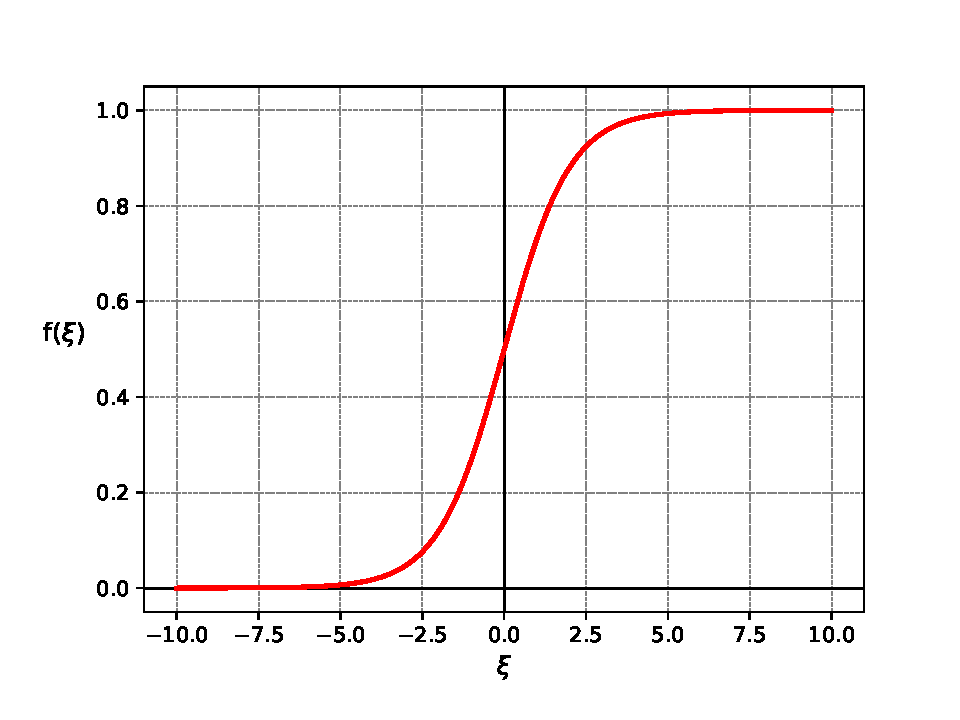
\includegraphics[width=1\textwidth]{../img/graph_sigmoid.pdf}
        \caption{Funkce \emph{sigmoida}}
        \label{fig:graph_sigmoid}
    \end{minipage}%
    \begin{minipage}{0.5\textwidth}
        \centering
        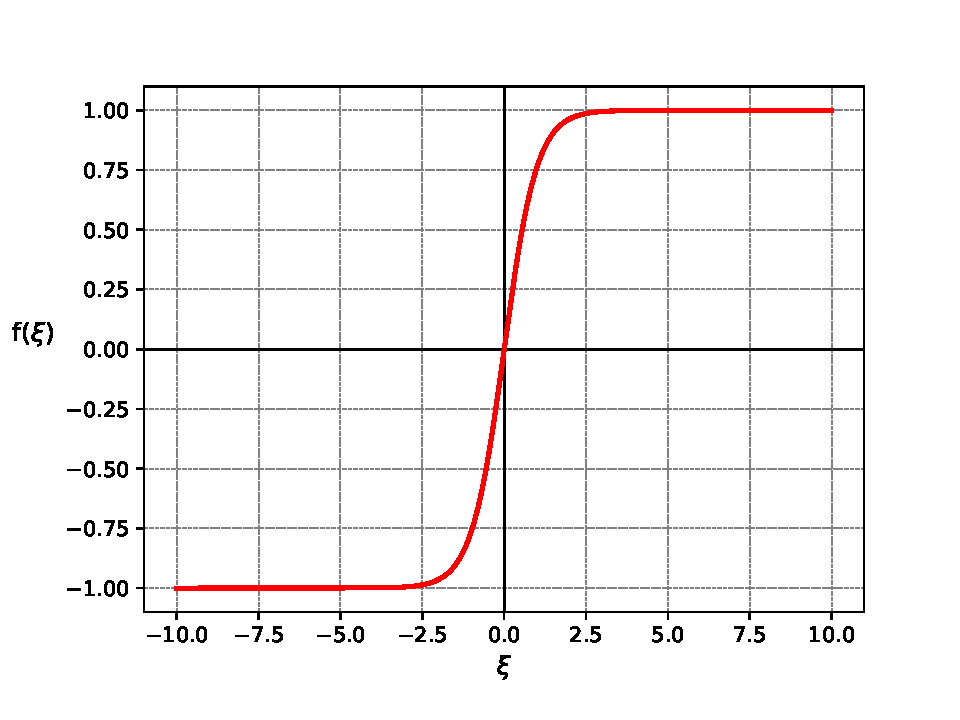
\includegraphics[width=1\textwidth]{../img/graph_tanh.pdf}
        \caption{Funkce \emph{tanh}}
        \label{fig:graph_tanh}
    \end{minipage}
    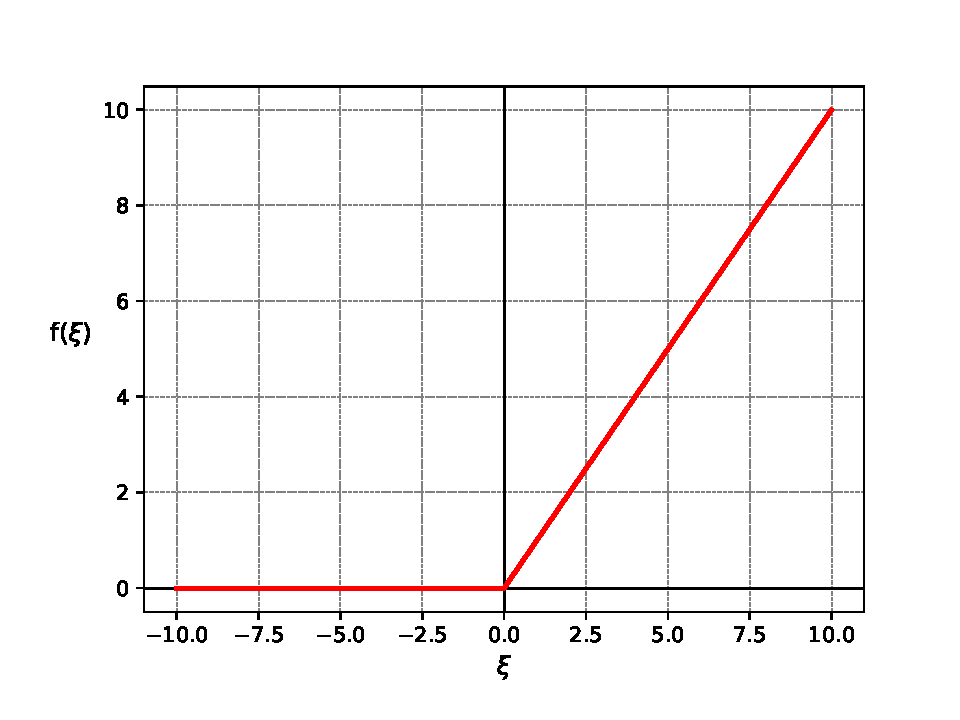
\includegraphics[width=0.5\textwidth]{../img/graph_relu.pdf}
    \caption{Funkce \emph{ReLU}}
    \label{fig:graph_relu}
\end{figure}

\paragraph{Neuronová síť}
Architektura neuronové sítě je tvořena ze třech základních typů neuronů --
vstupních (ze kterých pouze vycházejí spojení), výstupních (do kterých pouze
přicházení spojení) a skrytých (mají vstupní i výstupní spoje). Neuronová síť
se pak dá popsat jako orientovaný graf. Pokud se jedná o graf bez orientovaných
cyklů můžeme síť označit za \emph{dopřednou neuronovou síť}. Pokud obsahuje
nějaké orientované cykly, označujeme ji jako \emph{rekurentní neuronovou síť}.
Dále se budeme zaměřovat na \emph{dopředné vrstevnaté neuronové sítě}.

Dopředné neuronové sítě jsou často rozdělené do vrstev a nazývají se vrstevnaté
neuronové sítě. V těchto sítích vstup přechází po orientovaných hranách
vrstvami neuronů, kde každý neuron z předchozí vrstvy je spojen hranou s každým
vrcholem v následující vrstvě. První vrstva se nazývá \emph{vstupní vrstva}. Je
tvořena ze \emph{vstupních neuronů} a slouží pro vstup parametrů (vstupů) do
sítě. Vstupní neuron dostane hodnotu konkrétního vstupu a tuto hodnotu posílá
beze změny dále (vstupní neurony nepoužívají aktivační funkci). Poslední vrstva
se nazývá \emph{výstupní vrstva}. Je tvořena z \emph{výstupních neuronů} a
výstup těchto neuronů je zároveň výstupem celé sítě. Každá neuronová síť musí
nutně mít alespoň jeden vstupní a alespoň jeden výstupní neuron. Libovolná
další vrstva mezi \emph{vstupní} a~\emph{výstupní vrstvou} se nazývá
\emph{skrytá vrstva}. Těchto vrstev může být v síti teoreticky libovolné
množství.

Následující rovnice předvedou jeden dopředný průchod neuronovou sítí
transformující vstupní vektor hodnot na výstupní vektor. V tomto příkladu si
představíme průchod dat jednoduchou sítí, skládající se ze vstupní vrstvy
(výstupy $n$~vstupních neuronů značíme $x_1,...,x_n$), jedné skryté vrstvy
neuronů (výstupy $k$~neuronů v této vrstvě označíme $h_1,...,h_k$, s
odpovídajícím vektorem prahů $b_1,...,b_k$ a~váhami $w_{j,i}$ pro $j=1,...,n$ a
$i=1,...,k$) a výstupní vrstvy (výstupy $m$ neuronů výstupní vrstvy označíme
jako $y_1,...,y_m$, matici vah $w'_{j,i}$ pro $j=1,...,k$ a~$i=1,...,m$ a
vektor prahů $b'_1,...,b'_m$).

Výstup skrytých neuronů se spočítá jako,
\begin{equation} \label{eq:hidden}
    h_i = f(\sum_{j=1}^{n} x_j w_{j,i} + b_i), \quad i = 1,...,k
\end{equation}
kde $w_{j,i}$ je váha hrany ze vstupního neuronu $j$ do skrytého neuronu $i$ a
$f$ je aktivační funkce neuronů skryté vrstvy.
Výstupy výstupních neuronů se spočítají jako,
\begin{equation} \label{eq:output}
    y_i = a(\sum_{j=1}^{k} h_j w'_{j,i} + b'_i), \quad i = 1,...,m
\end{equation}
kde $w'_{j,i}$ je váha hrany z $j$-tého skrytého neuronu do $i$-tého výstupního
neuronu a $a$ je aktivační funkce neuronů výstupní vrstvy.

\paragraph{Trénování neuronových sítí}
Trénování (neboli učení) neuronových sítí je často velmi složitý proces, při
kterém se snažíme nastavit hodnoty vah jednotlivých spojů mezi neurony tak,
abychom pro konkrétní vstup na \emph{vstupní vrstvě}, dostali požadovaný výstup
na \emph{výstupní vrstvě}. 

Toto je nejčastější požadavek pro neuronové sítě při tzv. \emph{učení s
učitelem} (\emph{supervised learning}). Při tomto učení síť dostává dvojice
vektorů $(x, t)$, kde $x$~je vektor vstupních hodnot a $t$ je vektor
požadovaných výstupů. Následně se $x$~nastaví jako potenciál vstupních neuronů
a síť spočítá výstupy na výstupních neuronech. Vektor výstupních neuronů
(obvykle značený $y$) se porovná s požadovaným výstupem $t$. Na základě rozdílů
(chyby) těchto hodnot se provede úprava vah jednotlivých spojů tak, aby se při
opakovaném výpočtu sítě chyba zmenšila. Tohoto lze dosáhnout často používaným
algoritmem zpětného šíření chyby (\emph{backpropagation}), který počítá
derivace chybové funkce podle vah tak, aby vždy prováděl úpravy vah spojů ve
směru klesající chybové funkce.

Tento přístup ale přestává fungovat, pokud nedokážeme vytvořit vstupní
trénovací dvojice \emph{(vstup, požadovaný výstup)}, a tedy bychom nevěděli jakým
směrem váhy spojů upravovat. Toto je překážka v mnoha praktických problémech,
na které by se neuronové sítě hodilo použít. Možným řešením je nevyužívat učící
metody založené na propagaci výsledné chyby sítě, ale použít nějakou hodnotící
funkci, která ohodnotí kvalitu konfigurace dané sítě (např. po simulačním
běhu). Toto nás vede k možnosti využití evolučních algoritmů pro trénovaní
neuronových sítí evolučním algoritmem.

\section{Neuroevoluce} \label{NN - evolve}
Neuroevoluce \citet{Lehman:2013} je technika pro evoluční vývoj umělých
neuronových sítí pomocí principů evolučních algoritmů (popsaných sekci
\ref{Evoluční algoritmy}). Vývoj pomocí neuroevoluce je obecnější než vývoj
pomocí klasických trénovacích metod, jelikož vývoj, na rozdíl od trénovacích
metod založených na principu \emph{učení s učitelem}, může probíhat i na sítích
proměnlivé architektury a~nepotřebuje znát korektní výstupy pro daný vstup
sítě. Pro trénovaní stačí, když~jsme schopni nějakým způsobem ohodnotit kvalitu
řešení, k jakému se s využitím dané konfigurace (architektura, váhy spojení a
prahy) sítě dostaneme. Díky tomuto se neuroevoluce hodí pro vývoj neuronových
sítí v případech, kdy nejsme schopni přesně určit správné výstupy sítě pro dané
vstupy a pouze můžeme pozorovat kvalitu chování daného vyvíjeného systému.

\paragraph{Vývoj neuronových sítí}
Vývoj pomocí neuroevoluce probíhá stejně jako u~jiných evolučních algoritmů.
Neuronová síť je zakódovaná do genotypu jedinců, množina těchto jedinců potom
tvoří populaci, procházející vývojem skrz opakované generace. V každé generaci
je genotyp každého jedince dekódován a z těchto informací je vytvořena
neuronová síť podle dekódované architektury a vah spojení. Pro každého jedince
je jeho dekódovaná síť následně otestována v testovacím prostředí, kde se
ohodnotí kvalita jedince (fitness).

Jednoduchým typem kódování může být uložení hodnot vah všech hran v~neuronové
síti do jediného vektoru. Takový vektor se použije jako genotyp jedince.
To~umožňuje optimalizaci vah sítě s fixní architekturou. Tento typ kódování
může být ale výpočetně velmi náročný, kvůli rychle narůstající délce genotypu s
velikostí architektury (počet vrstev a počet neuronů v síti) neuronové sítě.

\paragraph{Pokročilé metody}
Výše uvedené problémy můžeme řešit hned několika způsoby. Různé styly
zakódování neuronových sítí do genotypu umožňují vývoj mnohem
rozsáhlejších sítí, a přitom zachovávají udržitelně malou velikost genetické
informace jedinců. 

Některé metody \citet{gomez2008accelerated} navrhovaly postup, jakým můžeme
omezit vývoj z celých neuronových sítí na pouze menší komponenty, které dále
mohly být spojovány dohromady s ostatními jedinci v kooperativní evoluci. To
umožnilo evoluční vývoj sítí rozsáhlejších architektur s menšími nároky na
velikost genotypu.

Jiné metody se poté zaměřily na vývoj jak vah, tak topologie neuronové sítě.
Navíc se ukázalo, že současný vývoj topologie často přináší lepší výsledky
než~vývoj pouze vah sítě. Vývoj v těchto metodách začíná s nejzákladnější
strukturou sítě, která se podle nároků problému sama vyvíjí a rozšiřuje, dokud
tyto změny přináší kvalitativní zlepšení. Často využívaným algoritmem
využívající těchto metod je algoritmus NEAT (\emph{NeuroEvolution of Augmenting
Topologies}), který si představíme v následujícím oddílu.

\subsection{NEAT} \label{NN - NEAT}
NEAT (\emph{NeuroEvolution of Augmenting Topologies})
\citep{stanley2002evolving} je neuroevoluční algoritmus vyvíjející najednou
váhy synapsí i topologii neuronové sítě, který se díky své výkonnosti stal
jedním z nejznámějších algoritmů používaných pro účely evolučního vývoje
neuronových sítí. Autoři jeho efektivitu připisují třem základním principům, se
kterými algoritmus pracuje:
\begin{enumerate}
    \item značkování genetických informací pomocí tzv. \emph{historických značek},
        umožňující smysluplné křížení genotypů napříč různými topologiemi,
   \item ochrana nových genetických informací v populaci pomocí rozdělení\\
       do druhů,
    \item postupný vývoj topologie sítí od nejjednodušších struktur ke
        složitějším.
\end{enumerate}
S těmito principy se NEAT ukázal jako algoritmus, který často nachází efektivní
sítě rychleji než ostatní algoritmy a výkony překonal nejlepší neuroevoluční
algoritmy pracující s neuronovými sítěmi s fixní topologií.

\paragraph{Algoritmus}
NEAT používá tzv. \emph{přímé kódování}, tedy genotyp každého jedince přímo
popisuje celou topologii sítě (všechny neurony a všechny hrany mezi neurony).
Každý genotyp obsahuje seznam \emph{genů synapsí} a seznam \emph{genů neuronů}.
\\Seznam genů neuronů popisuje vstupní, výstupní a skryté neurony sítě,
které~mohou být spojené hranami. Každý gen synapse obsahuje následující
informace: 
\begin{itemize}
    \item koncový neuron -- neuron, do kterého synapse vchází,
    \item počáteční neuron -- neuron, ze kterého synapse vychází,
    \item hodnotu váhy synapse,
    \item příznak, jestli je spojení v síti použito,
    \item \emph{historická značka} -- číslo popisující kdy v historii
        byla daná hrana do sítě přidána; umožňuje nacházet
        odpovídající geny synapsí při křížení.
\end{itemize}
Algoritmus začíná s nejzákladnější strukturou, připomínající jednoduchý
perceptron, pouze s předem daným počtem vstupních a výstupních neuronů a
hranami mezi nimi. Tato jednoduchá topologie je rozšiřována pomocí
následujících genetických operátorů.

\paragraph{Mutace}
Mutace v algoritmu NEAT má schopnost měnit jak spojení v síti, tak~její
strukturu. Mutace synapsí sítě zahrnují jednoduchou změnu váhy spojení nebo
změnu příznaku použití daného spojení v síti. Struktura sítě může mutovat dvěma
způsoby. První typ mutace přidává nový gen synapsí, spojující dva doposud
nespojené neurony. Druhý typ mutace přidává nový neuron. Tato mutace probíhá
tak, že na místo existující synapse se přidá nový neuron. Původní synapse se
označí jako nepoužívaná a namísto toho se vytvoří dvě nové rozdělující tu
původní. Váha spojení je v tomto procesu zachována. Při těchto operacích je
vždy novým genům synapsí přiřazena nová \emph{historická značka} (používá se
globální čítač, jehož číslo je s každým novým genem navýšeno). Růst sítí
probíhá právě díky mutaci.

\paragraph{Křížení}
Křížení využívá \emph{historické značky}. Dva jedinci se nejdříve hranami
zarovnají pomocí jejich \emph{historických značek}. Stejná čísla historických
značek totiž v~síti značí stejnou strukturu. Synapse, která se v obou jedincích
shoduje (má stejnou historickou značku) se dědí náhodně z jednoho rodiče.
Synapse, kterou má jen jeden z rodičů se dědí pouze když je v lepším z rodičů a
pokud je v nějakém jedinci hrana neaktivní a~v~druhém aktivní, s danou
pravděpodobností se tento stav v novém jedinci změní. Algoritmus je tímto
stylem schopný vytvářet velké množství různých topologií. Tyto nové topologie,
přestože jsou často důležité pro řešení zadaného problému, mají jen velmi malou
šanci se v populaci menších topologií udržet, protože původní menší topologie
jsou v době vzniku větší topologie často optimalizovanější než tyto nové
topologie. Proto NEAT využívá systém, kterým chrání tyto nové topologie před
vyhynutím z populace.

\paragraph{Ochrana nových druhů}
Nové topologie jsou chráněny rozřazením genotypů do odlišných druhů. Jednotlivé
genotypy poté primárně soutěží s jedinci stejného druhu a nové druhy tak mají
šanci se vyvinout a optimalizovat na jejich úroveň. NEAT pro výpočet odlišností
jedinců opět využívá \emph{historické značky}, pomocí kterých hledá společné
hrany a vypočítá vzdálenost dvou genomů. Geny obou jedinců rozdělíme do
několika kategorií. Buď se shodují (mají stejnou \emph{historickou značku}),
a~pak jsou označené jako shodné (\emph{matching genes}), nebo se neshodují.
Neshodné geny, které~mají historické značky v rozmezí hodnot \emph{historických
značek} druhého z~jedinců, se nazývají disjunktní (\emph{disjoint}) a zbylé
geny se nazývají přesahující (\emph{excess}). Hodnota vzdálenosti dvou jedinců
se poté počítá jednoduchou lineární kombinací počtu genů jako:

\begin{equation}
    \delta = \frac{c_1E}{N} + \frac{c_2D}{N} + c_3\cdot\overline{W}
\end{equation}
kde $N$ je celkový počet genů ve větším z jedinců, $E$ je počet přesahujících
genů, $D$ je počet disjunktních genů, $\overline{W}$ je průměrný rozdíl vah
shodujících se genů a~koeficienty $c_1$, $c_2$ a $c_3$ umožňují nastavovat
důležitost těchto tří faktorů \citep{stanley2002evolving}.

Na začátku generace se pak vytváří seznam druhů. Pokud se objeví genom, který
nezapadá do žádného z druhů, je pro něj vytvořen jeho vlastní nový druh.

\paragraph{Fitness}
Rozdělení do druhů má vliv i na fitness jedinců. Kvalita každého jedince se při
výpočtu fitness dělí počtem jedinců stejného druhu (vzorec
(\ref{eq:neatfitness})). To~zároveň omezuje druhy v ovládnutí celé generace a
dál ochraňuje nové topologie.
\begin{equation} \label{eq:neatfitness}
    f'_i = \frac{f_i}{\sum_{j=1}^n sh(\delta(i,j))}
\end{equation}
kde $sh$ je binární indikátor s hodnotou 1, pokud je vzdálenost $\delta(i,j)$
menší než daný práh $\delta_t$, jinak má hodnotu 0. $f_i$ je fitness hodnota
jedince a $f'_i$ jeho upravená hodnota.

\paragraph{Minimalizace dimenzionality jedinců}
Jak již bylo zmíněno, NEAT inicializuje celou populaci jedinců s minimální
topologií, obsahující pouze nutný počet vstupních a výstupních neuronů,
které jsou navzájem plně propojené a neobsahuje žádné skryté neurony. Nové
topologie vznikají díky genetickým operátorům a~všechna zvětšení genotypů jsou
tedy v evoluci opodstatněná. Díky tomuto NEAT samovolně vede k vývoji
minimálních topologií. To umožňuje, že tento algoritmus je často výkonnější než
ostatní, protože prohledává minimální potřebný prostor pro nalezení řešení,
oproti neuroevolučním algoritmům, které používají fixní topologie neuronových
sítí.

\subsection{HyperNEAT} \label{NN - HyperNEAT}
Pro porovnání uvádíme jeden pokročilejší algoritmus. Algoritmus HyperNEAT
(\emph{Hypercube-based NEAT}) \citep{stanley2009hypercube} \citep{eplex} je
neuroevoluční algoritmus rozšiřující algoritmus NEAT. HyperNEAT slouží pro
vývoj umělých neuronových sítí fixní topologie. 

Na rozdíl od algoritmu NEAT, používá HyperNEAT nepřímou
reprezentaci vah sítě. Tyto váhy jsou reprezentovány pomocí jiné neuronové
sítě (\emph{Compositional Pattern-Producing Network}, zkráceně \emph{CPPN}),
která jako vstup dostává pozice dvou neuronů v prostoru a vrací váhu jejich
spojení (synapse). Tímto stylem může \emph{CPPN} být využita pro reprezentaci
sítě libovolné topologie. 

Síť \emph{CPPN} je poté v algoritmu HyperNEAT vyvíjena pomocí NEAT.

Díky této nepřímé reprezentaci vah má HyperNEAT schopnost efektivně vyvinout
velmi rozsáhlé neuronové sítě s předem určenou strukturou (takto dokáže např.
napodobit regularitu velkého množství spojů v lidském mozku).

\paragraph{}
Naznačení průběhu HyperNEAT algoritmu:
\begin{enumerate}
    \item Zvolit konfiguraci vyvíjené sítě (vstupní a výstupní neurony a
        rozložení skrytých neuronů).
    \item Inicializovat NEAT algoritmus s \emph{CPPN} sítěmi.
    \item Běh NEAT algoritmu, dokud není nalezeno řešení:
        \begin{enumerate}
            \item pomocí \emph{CPPN} daného jedince vytvoř synapse pro původní
                síť,
            \item síť otestuj v testovacím prostředí pro výpočet kvality
                řešení,
            \item s fitness hodnotami pokračuj ve vývoji genotypů popisujících
                \emph{CPPN} sítě.
        \end{enumerate}
\end{enumerate}

Protože v práci nebudeme HyperNEAT používat, detailnější popis vynecháme.

\section{Simulované prostředí} \label{Simulované prostředí}

Jelikož chceme vyvíjet řízení robotů založené na interakcích s prostředím,
je~pro tuto práci důležité vybrat vhodný simulátor prostředí. Například při
vývoji počítačových her se využívají různé výpočetně výhodné simulátory
prostředí. My však chceme, aby se chování objektů v simulátoru virtuálního
prostředí co nejvíce blížilo chování objektů v reálném prostředí. Proto budeme
využívat pouze robustní simulátory prostředí, založené na fyzikálních zákonech.
Budeme rozlišovat mezi \emph{simulátorem prostředí}, který eviduje objekty (a
vlastnosti objektů jako třeba rozměry, váha atd.), a \emph{simulátorem
fyziky}, který řeší interakce mezi objekty tak, aby odpovídaly fyzikálním
zákonům. 

Přáli bychom si mít možnost jednoduše konfigurovat co nejvíce vlastností
prostředí a zároveň mít co nejjednodušší přístup k morfologii simulovaných
robotů. Zároveň chceme, abychom měli možnost do morfologie robotů nějakým
způsobem zasahovat i v průběhu evolučního vývoje a aktivně ji za běhu měnit.
Jelikož plánujeme v různých prostředích provádět experimenty s různými typy
robotů, používajícími různé styly pohybu (typy motorů, kloubů, tvarů končetin
atd.), je~potřebné, aby fyzikální simulátor (\emph{fyzikální řešič=solver}) byl
schopný simulovat i složitější typy robotů. Takovými mohou být právě třeba
kráčející roboti neboli roboti používající k pohybu končetiny připomínající
nohy, na rozdíl od jednodušších typů robotů, kteří se mohou pohybovat pomocí
kol, jejichž simulace bývá mnohdy jednodušší. 

Stejně tak, jak potřebujeme umožnit simulaci složitějších robotů, protože
nebudeme mít možnost vlastnoručně kontrolovat každý parametr, který bude při
vývoji robotům přiřazen, potřebujeme zajistit, aby fyzikální simulátor zvládal
velké rozsahy parametrů a simulace zůstala s těmito parametry stabilní. Zároveň
chceme, aby simulátor v prostředí byl deterministický, což umožní, že
předváděné experimenty můžeme dle potřeby opakovat a výsledky tak náležitě
prezentovat. 

Evoluční algoritmy jsou velmi lehce paralelizovatelné a tedy pro
urychlení procesu vývoje a experimentů bude pro nás výhodné, pokud by simulace
zvládala paralelní běh na více vláknech (více simulací, každá na vlastním
vlákně). V neposlední řadě pro lehčí integraci do vlastního modulu bude
užitečné, aby modul spravující zvolený simulátor byl open-source, což nám dá
volnost v případě, že si budeme chtít chování systémů v prostředí nějak
vlastnoručně upravit.

V oddíle \ref{Simulátory prostředí} popíšeme několik simulátorů prostředí,
které využívají fyzikální simulátory. Samotné fyzikální simulátory představíme
v oddíle \ref{Fyzikální simulátory}.

\subsection{Simulátory prostředí} \label{Simulátory prostředí}

Při hledání simulátorů prostředí, které by vyhovovali našim požadavkům
a zároveň umožňovali kontrolu a ovládání prostředí prostřednictvím zvoleného jazyka
Python, jsme narazili na několik možností. Omezený výčet těchto simulátorů zde
popíšeme -- Gazebo (v oddílu \ref{Gazebo}), Webots (v oddílu \ref{Webots}) a
CoppeliaSim (v oddílu \ref{CoppeliaSim}).

\subsubsection{Gazebo} \label{Gazebo}
Gazebo \citep{gazeborobotics} je sada open-source víceplatformních knihoven pro
vývoj, výzkum a aplikaci robotů, která vznikla v roce 2002. Umožňuje kompletní
kontrolu nad simulací dynamického 3D prostředí s více agenty a generování dat
ze simulovaných senzorů. Fyzikálně korektní interakce v prostředí pak od
začátku projektu zajišťuje známý fyzikální simulátor ODE (viz sekce \ref{ODE}),
nad kterým Gazebo tvoří abstraktní vrstvu, umožňující snazší tvorbu
simulovaných objektů různých druhů. V dnešní době je stále výchozím fyzikálním
simulátorem ODE, nicméně uživatel si již může vybrat celkem ze čtyř různých
fyzikálních simulátorů -- Bullet (sekce \ref{Bullet}), Simbody, Dart (sekce
\ref{Dart}) a ODE. Uživatel s knihovnou pracuje prostřednictvím grafického
rozhraní založené na knihovně Open Scene Graph používající OpenGL, nebo
prostřednictvím příkazové řádky. Prostředí a~roboti mohou být tvořené buď z
grafického rozhraní prostředí, nebo~v~textovém formátu XML. Limitací Gazebo je
pak chybějící možnost rozdělit simulace mezi vícero vláken kvůli vnitřní
architektuře spojené s fyzikální simulací \citep{koenig2004design}. 

\subsubsection{Webots} \label{Webots}
Webots \citep{Webots} je open-source víceplatformní, robustní a deterministický
robotický simulátor vyvíjený od roku 1998. Umožňuje programování a testování
virtuálních robotů mnoha různých typů a jednoduchou následnou aplikaci softwaru
v reálných robotech. Simulátor je možné použít pro simulaci prostředí s~vícero
agenty najednou. Agenti spolu mohou komunikovat, a to jak lokálně, tak
i~globálně. Výpočty fyzikálních interakcí zajišťuje fyzikální simulátor ODE.
Pro vývoj robotů a prostředí je možné využít řady programovacích jazyků a to C,
C++, Python, Java, MATLAB nebo ROS (\emph{Robot Operating System}). Prostředí
umožňuje práci v grafickém rozhraní a vizualizaci simulací pomocí OpenGL.
Knihovna dále nabízí využití připravených modelů robotů, vlastní editor robotů
a map a~možnosti vložení vlastních robotů z 3D modelovacích softwarů v CAD
formátu \citep{michel2004cyberbotics}.

\subsubsection{CoppeliaSim} \label{CoppeliaSim}
CoppeliaSim \citep{coppeliaSim} \citep{coppeliarobotics} (původně známý pod
jménem \emph{V-REP} = \emph{Virtual Robot Experimentation Platform}) je
víceplatformní simulační modul pro vývoj, testování a jednoduchou aplikaci
softwaru pro roboty. Dovoluje vývoj ovladačů pomocí 7 různých programovacích
jazyků a ulehčuje jejich aplikace v simulovaných a skutečných robotech.
Simulaci ovladačů je možno jednoduše rozdistribuovat mezi vícero vláken dokonce
vícero strojů, což urychluje vývoj a snižuje nároky na procesor v době
simulace. Navíc je možné vyvíjený ovladač nechat v době simulací běžet na
samotném (bezdrátově) připojeném robotovi, co dále ulehčuje přenos finální
verze ovladačů z vývoje do reálného světa. Prostředí umožňuje práci s
širokou řadou typů objektů, druhů kloubů, senzorů a dalších objektů obvykle
používaných při vývojích robotických ovladačů. Obsahuje snadno použitelný
editor prostředí a robotů samotných s řadou předem vytvořených modelů, které
může uživatel hned využít. Modely zároveň mohou být přidány v řadě různých
formátů (XML, URDF, SDF). Prostředí podporuje pět různých fyzikálních
simulátorů (Bullet, ODE, MuJoCo (v sekci \ref{MuJoCo}), Vortex (v sekci
\ref{Vortex}) a Newton), mezi kterými si uživatel může vybrat dle potřeb
přesnosti (reálnosti), rychlosti a dalších možností jednotlivých fyzikálních
simulátorů \citep{nogueira2014comparative}.

\subsection{Fyzikální simulátory} \label{Fyzikální simulátory}

V této podkapitole se podíváme na základní popis a možné výhody a nevýhody
jednotlivých fyzikálních simulátorů, na které jsme narazili při hledání
simulátorů prostředí.

\subsubsection{ODE} \label{ODE}
ODE (\emph{Open Dynamics Engine}) \citep{opendynamicsengine} je víceplatformní
open-source fyzikální simulátor, jehož vývoj začal v roce 2001. Je vhodný pro
simulaci pevných těles s různými druhy kloubů a pro detekci kolizí. Byl navržen
pro využití v interaktivních nebo real-time simulacích, upřednostňujících
rychlost a stabilitu nad fyzikální přesností \citep{smith2007open}. Kvůli
stabilitě vyžaduje používání menších simulačních kroků. Hodí se pro simulaci
vozidel, kráčejících robotů a virtuálních prostředí. Má široké využití v
počítačových hrách a 3D simulačních nástrojích jako jsou CoppeliaSim (v sekci
\ref{CoppeliaSim}), Gazebo (v sekci \ref{Gazebo}), Webots (v sekci
\ref{Webots}) a dalších.

\subsubsection{Bullet} \label{Bullet}
Bullet je open-source fyzikální knihovna, podporující detekci kolizí a simulaci
pevných a měkkých těles. Bullet je používán jako fyzikální simulátor pro hry,
vizuální efekty a robotiku \citep{coumans}. Byl použit jako hlavní fyzikální
simulátor pro simulaci NASA \emph{Tensegrity} robotů (s vlastními úpravami pro
simulaci měkkých těles, kvůli nerealistickým metodám řešení simulace provazů)
\citep{izadi2018simulating}.

\subsubsection{Dart} \label{Dart}
Dart (\emph{Dynamic Animation and Robotics Toolkit}) je víceplatformní otevřená
knihovna pro simulace a animace robotů. Od předchozích se odlišuje stabilitou
a~přesností, díky zobecněné reprezentaci souřadnic pevných těles v simulaci.
Na~rozdíl od ostatních fyzikálních simulátorů, aby dal vývojáři plnou kontrolu
nad simulací, umožňuje Dart plný přístup k interním hodnotám simulace. Zároveň
se díky línému vyhodnocování hodí pro vývoj real-time ovladačů pro roboty
\citep{lee2018dart}.

\subsubsection{MuJoCo} \label{MuJoCo}
MuJoCo (\emph{Multi-Joint Dynamics with Contact}) \citep{deepmind_2021} je
open-source fyzikální simulátor pro vývoj v oblasti robotiky, biomechaniky a
dalších. Často je využíváno pro testování a porovnávání různých metod
navrhování robotických systémů jako jsou třeba evoluční algoritmy nebo metody
zpětnovazebného učení \citep{salimans2017evolution}. V simulacích je pro roboty
možné nakonfigurovat využití mnoha druhů aktuátorů, včetně těch simulujících
práci svalů a k dispozici je i velké množství kloubů. Simulátor zároveň
umožňuje velký nárůst v rychlosti běhu simulace za pomoci plné podpory
paralelizace na všech dostupných vláknech a dobrou stabilitu simulace i při
velmi velkých simulačních krocích \citep{todorov2012mujoco}. Zároveň nabízí
jednoduchý styl, jakým si může uživatel konfigurovat všechny detaily simulace a
samotných simulovaných robotů pomocí jednoduchých XML konfiguračních souborů
(XML formát modelů \emph{MJCF}). V komplexním rozboru řady často používaných
fyzikálních simulátorů byl simulátor MuJoCo hodnocen jako jeden z nejlepších co
se týče stability, přesnosti a rychlosti simulací. Další výhodou zlepšující
přesnost tohoto simulátoru je, že MuJoCo pro simulaci používá kloubní
souřadnicový systém, který předchází porušování fyzikálních pravidel a tedy
nepřesností v kloubech \citep{erez2015simulation}.

\subsubsection{Vortex} \label{Vortex}
Vortex je uzavřený, komerční fyzikální simulátor určený pro tvorbu
reálnému světu odpovídajících simulací. Obsahuje mnoho parametrů,
umožňující nastavení reálných fyzikálních parametrů dle potřeb,
většinou industriálních a výzkumných aplikací \citep{coppeliarobotics}
\citep{yoon2023comparative}.

\subsubsection{Porovnání simulátorů} \label{Simulátory - Porovnání}
V dnešní době se nám nabízí velké množství potencionálních kandidátů, vhodných
k využití pro naši aplikaci. Každý z open-source simulátorů, které jsme našli a
představili, by bylo možné použít pro simulaci robotů složitosti, jakou~máme
předběžně v plánu. Hlavním z rozhodujících faktorů pro tento projekt bude, jak
jednoduše půjde prostředí používat pro vývoj pomocí genetických algoritmů.
Chceme tedy nějaký jednoduchý přístup k simulaci a ovládání robotů, rychlost
a~přesnost simulace. 

Opět většina ze simulátorů prostředí toto nabízí. Osobně se nám ale nejvíce
zalíbilo MuJoCo. Díky nedávnému převedení fyzikálního simulátoru MuJoCo do
open-source a změně prostředí (nejprve do \textbf{OpenAI Gym} a nyní do
\textbf{Farama Foundation Gymnasium}) jsme dostali možnost využít jednoduché
Python API pro ovládání robotů a zároveň konfiguraci celé simulace. 

Tato abstrakce od vlastní simulace je pro tuto práci velmi přínosná, protože~se
především chceme zajímat o vývoj řízení robotů pomocí evolučních algoritmů.
Řešit zároveň složité ovladače robotů, které by se mohly lišit pro různé typy
robotů, by mohlo bezdůvodně komplikovat celý proces spojení evolučních
algoritmů s řízením robotů. Takové věci by pak mohly být problematické pro
možného uživatele, který by si chtěl sám evoluční algoritmy upravovat.

MuJoCo se zároveň ukazuje jako jeden z nejlepších volně dostupných fyzikálních
simulátorů dnes. Z výsledků článku testujících různé vlastnosti známých fyzikálních
simulátorů \citet{erez2015simulation} vychází, že MuJoCo má navrch jak
v~rychlosti, tak ve kvalitě simulací. Zároveň interně využívá kloubní
souřadnicový systém, který je přesnější, protože zabraňuje nepřesnostem v
kloubech. To~se hodí o to více, když v této práci chceme vyvíjet hlavně
kráčející roboty, u kterých můžeme mít i větší počty kloubů. 

Simulátor MuJoCo a roboti, které můžeme používat, je zároveň možné
jednoduše konfigurovat pomocí vlastního XML formátu a spojení s Python API
navíc umožní tyto konfigurace provádět, jak často bude potřeba.
